\documentclass[t]{beamer}
\usepackage{color}
\usepackage{amsmath}
\usepackage{pdfpages}

\definecolor{dkgreen}{rgb}{0,0.5,0}
\definecolor{gray}{rgb}{0.5,0.5,0.5}
\definecolor{Maroon}{rgb}{0.6,0,0}
\newcommand\df{\bf\color{Maroon}}
\newcommand\dff{\bf\color{dkgreen}}
\setbeamercolor{background canvas}{bg=}
\usetheme{TuringLight}
%\usetheme{TuringDark}

% Presentation data
\title{\color{Maroon} MLJ Workshop}
\subtitle{{\small Resources: \bfseries{github.com/ablaom/MLJTutorial}}}
\date{July, 2020}
\author{Anthony Blaom with Quinn Asena}

% Uncomment any of these lines below to set custom size for each of the font sizes.
% The default value is shown in the comment.
%\setlength{\titlefontsize}{6.875\basefontsize}
%\setlength{\subtitlefontsize}{4.375\basefontsize}
%\setlength{\frametitlesize}{2.625\basefontsize}
%\setlength{\framesubtitlesize}{1.625\basefontsize}
%\setlength{\bodytextsize}{2\basefontsize}
%\setlength{\blocktitlesize}{\bodytextsize}
%\setlength{\blockbodysize}{\bodytextsize}

% Start document
\begin{document}


% Title slide (details filled from presentation data fields above)

% \begin{frame}
%   \frametitle{Installing the tutorials}

%   Please follow instructions at:
%   \begin{center}
%     {\df github.com/ablaom/MachineLearningInJulia2020}
%   \end{center}
% \end{frame}

\begin{frame}
        \titlepage
\end{frame}

\begin{frame}
  \vspace{0\baselineskip}
  \begin{center}
    \includegraphics[scale=0.2]{Turing_logo.png}
    \includegraphics[scale=0.35]{UoA_logo.png}

    \includegraphics[scale=0.2]{IQVIA_logo.png}
    \includegraphics[scale=0.12]{NESI-logo.jpg}
    \includegraphics[scale=0.12]{warwick.png}
    \includegraphics[scale=0.12]{julia.png}
  \end{center}
\end{frame}

\begin{frame}
  \frametitle{The Team}

  {\small
    {\dff Core design:} A. B., Franz Kiraly, Sebastian Vollmer\\[1\baselineskip]

    {\dff Lead development:} A. B., Thibaut Lienart \\[1\baselineskip]

    {\dff Other contributors:} Diego Arenas, Samuel Okon, Yiannis Simillides, Julian Samaroo, Ayush Shridar, Geoffroy Dolphin, Mosè Giordano\ldots \\[1\baselineskip]

    {\dff Julia language consultants:} Avik Sengupta\\[1\baselineskip]}

\end{frame}

% \begin{frame}
%   \frametitle{Contributing}
%   \begin{itemize}
%      \item Star the MLJ.jl repo!
%      \item Report problems by raising issues
%      \item Contribute a tutorial at DataScienceTutorials.jl
%      \item Implement the MLJ interface new models
%      \end{itemize}
% \end{frame}

% \begin{frame}
%   \frametitle{Interacting}
%    Zoom Webinar provides {\bf two} ways to interact:

%   \begin{block}{Q/A}
%     For asking panelists questions
%   \end{block}

%   \begin{block}{Chat}
%     For discussion {\em not} monitored by panelists
%   \end{block}\pause

%   \begin{block}{\includegraphics[scale=0.1]{raise_hand_forbidden.png}}
%   \end{block}

% \end{frame}

% \begin{frame}
%   \frametitle{Who?}
%   \begin{block}{Prerequisites:}\pause
%     \begin{itemize}
%     \item familiar with machine learning principles
%     \item basic Julia skills
%     \item experience using DataFrames or similar a plus
%     \end{itemize}
%   \end{block}
% \end{frame}

\begin{frame}
  \frametitle{Some machine learning libraries in Julia}
   \begin{center}
    \includegraphics[scale=0.2]{ML_packages_in_julia.png}
   \end{center}
\end{frame}

\begin{frame}
  \frametitle{Some multi-paradigm machine learning toolboxes in Julia}
  \begin{itemize}
  \item {\df ScikitLearn.jl} - thin wrapper for Python's scikit-learn
  \item {\df AutoMLPipeline.jl} - IBM
  \item {\df MLJ.jl}
  \item FastAI.jl - specific to neural networks (interface to {\df Flux.jl})
  \end{itemize}
\end{frame}

\begin{frame}
  \frametitle{What?}
  \begin{block}{What's a machine learning toolbox?}\pause
     \begin{itemize}
     \item A toolbox provides a {\df uniform interface} for {\df fitting}, {\df
         evaluating} and {\df tuning} machine learning models.
          \item Provides common {\df preprocessing tasks} (such as data cleaning
            and type coercion )
          \item Allows for model {\df composition} (e.g., pipelining)
      \end{itemize}
    \end{block}
\end{frame}

\begin{frame}
  \frametitle{Why?}
  \begin{block}{Why learn the MLJ toolbox?}
    \begin{itemize}
    \item Written in Julia (but does wrap non-native models):\pause
      \begin{itemize}
      \item Easy access to core algorithms
      \item Easier to customize
      \item Easier to add new performant models
      \item Greater transparency and reproducibility
      \item Better composability with other libraries\pause
      \end{itemize}
    \item Start-of-the-art {\df model composition} that plays well with everything else.
    \item Meta-algorithms (e.g., tuning) are model wrappers
    \end{itemize}
  \end{block}
\end{frame}

\includepdf[scale=1.3,pages={1,3}]{lego.pdf}

\begin{frame}
  \frametitle{Workshop Overview}
  \begin{itemize}

  \item Recap of supervised and unsupervised learning

  \item Preview of model composition (stacking)

  \item Part 1 - {\df Data Representation} + exercises

  \item Part 2 - {\df Selecting, Training and Evaluating Models} + exercises

  \item  Break

  \item Part 3 - {\df Transformers and Pipelines} + exercises

  \item Part 4 - {\df Tuning hyper-parameters} + exercises

  \item Part 5 - {\df Advanced model composition} (time permitting)

  \end{itemize}
\end{frame}

\begin{frame}
  \frametitle{Supervised Learning}
  Learning to {\df predict} some target variable {\df\large y} from a
  knowledge of some other variables {\df \large X} (the {\it input features}).\pause
  \begin{center}
    \includegraphics[scale=0.17]{X.png}\mbox{~~~~}
    \includegraphics[scale=0.17]{y.png}
  \end{center}
\end{frame}

\begin{frame}
  \frametitle{Supervised Learning}
   \begin{center}
    \includegraphics[scale=0.6]{overfitting1.png}
   \end{center}
\end{frame}

\begin{frame}
  \frametitle{Supervised Learning}
   \begin{center}
    \includegraphics[scale=0.6]{overfitting2.png}
   \end{center}
\end{frame}

\begin{frame}
  \frametitle{Supervised Learning}
   \begin{center}
    \includegraphics[scale=0.6]{overfitting3.png}
   \end{center}
\end{frame}

\begin{frame}
  \frametitle{Supervised Learning}
   \begin{center}
    \includegraphics[scale=0.6]{overfitting4.png}
   \end{center}
\end{frame}

\begin{frame}
  \frametitle{Supervised Learning}
   \begin{center}
    \includegraphics[scale=0.6]{overfitting5.png}
   \end{center}
\end{frame}

\begin{frame}
  \frametitle{Supervised Learning}
   \begin{center}
    \includegraphics[scale=0.6]{overfitting6.png}
   \end{center}
\end{frame}

\begin{frame}
  \frametitle{Unsupervised Learning}
  Learning data {\df transformations}, e.g., dimension reduction
   \begin{center}
    \includegraphics[scale=0.13]{PCA.png}
   \end{center}
\end{frame}

\begin{frame}
  \frametitle{Unsupervised Learning}
  Learning data {\df transformations}, e.g., dimension reduction
   \begin{center}
    \includegraphics[scale=0.13]{PCA2.png}
   \end{center}
\end{frame}

\begin{frame}
  \frametitle{Data science competitions (kaggle)}
  \vspace{-1.0\baselineskip}
    \begin{center}
      \includegraphics[scale=0.16]{kaggle1.png}
      \includegraphics[scale=0.16]{kaggle2.png}
      \includegraphics[scale=0.16]{kaggle3.png}
  \end{center}
\end{frame}

\begin{frame}
  \frametitle{Installing the tutorials}
  \vspace{4\baselineskip}
  \begin{center}
    \Large \df github.com/ablaom/MLJTutorial
  \end{center}
\end{frame}


\begin{frame}
        \finalpage
\end{frame}

\end{document}

\begin{frame}
  \frametitle{A plethora of models}
  \begin{center}
    \includegraphics[scale=0.08]{packages.jpg}
  \end{center}
\end{frame}

\begin{frame}
  \frametitle{Toolboxes in other ecosystems}
  \begin{center}
    \includegraphics[scale=0.4]{other_toolboxes.png}
  \end{center}
\end{frame}

\begin{frame}
  \frametitle{Goals for MLJ}\pause
  \begin{itemize}
  \item Want {\df usability}, interoperability,
       extensibility and reproducibility\pause
  \item Want avoid common {\df pain-points}:
    \begin{itemize}
       \item Identifying all models that solve a given task\pause
       \item Routine operations requiring a lot of code
%       \item Passage from data source to algorithm-specific
%         data format
%       \item Probabilistic predictions: evaluation, inconsistent representations
%       \item Limitations of {\df model composition} API \pause --- barrier to innovation!
    \end{itemize}
%  \item Hope that project adds some focus to Julia ML development more generally
  \end{itemize}
\end{frame}

%\begin{frame}
%   \frametitle{Advanced toolbox features}
%   \begin{block}{We want toolboxes that:}\pause
%     \begin{itemize}

%     \item Combine models in more flexible ways, e.g., ensembling,
%       stacking: pipelines $\rightarrow $ {\df learning
%         networks}.\pause
%     \item Avoid redundancies in retraining a learning network.\pause
%     \item Allow systematic tuning of nested parameters across a network\pause
%     \item Implement tuning as {\df model wrapper}\pause
%     \item Automatically match models to specified {\df tasks}
%   \end{itemize}
%   \end{block}
% \end{frame}

\begin{frame}
  \frametitle{Model search and tasks}
  \vspace{-1.5\baselineskip}
  \begin{center}
    \includegraphics[scale=0.38]{model_search1.png}
  \end{center}
\end{frame}

\begin{frame}
  \frametitle{Model search and tasks}
    \includegraphics[scale=0.30]{Sboston.png}
\end{frame}

\begin{frame}
  \frametitle{Quick performance evaluation}
  \includegraphics[scale=0.30]{Stree.png}
\end{frame}

\begin{frame}
  \frametitle{Quick performance evaluation}
  \includegraphics[scale=0.30]{Stree2.png}
\end{frame}

\begin{frame}
  \frametitle{Meta-algorithms as model wrappers}
  \includegraphics[scale=0.30]{Sforest.png}
\end{frame}

\begin{frame}
  \frametitle{Meta-algorithms as model wrappers}
  \includegraphics[scale=0.30]{Sforest2.png}
\end{frame}

\begin{frame}
  \frametitle{Meta-algorithms as model wrappers}
  \includegraphics[scale=0.30]{Sforest3.png}
\end{frame}

\begin{frame}
  \frametitle{Goals for MLJ}
  \begin{itemize}
  \item Want {\df usability}, interoperability,
       extensibility and reproducibility
  \item Want avoid common {\df pain-points}:
    \begin{itemize}
       \item Identifying all models that solve a given task
       \item Routine operations requiring a lot of code\pause
       \item Passage from data source to algorithm-specific
         data format
%       \item Probabilistic predictions: evaluation, inconsistent representations
%       \item Limitations of {\df model composition} API \pause --- barrier to innovation!
    \end{itemize}
%  \item Hope that project adds some focus to Julia ML development more generally
  \end{itemize}
\end{frame}

\begin{frame}
  \frametitle{Use any tabular data format}
  \vspace{-\baselineskip}
  \begin{center}
     \includegraphics[scale=0.25]{tableswordcloud.png}
  \end{center}
\end{frame}

\begin{frame}
  \frametitle{Scientific types}
  \vspace{-0.5\baselineskip}
  \begin{center}
    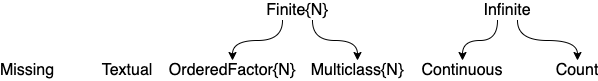
\includegraphics[scale=0.4]{scitypes.png}
  \end{center}%\pause
%  {\df Require:} Each julia object can represent only one scientific type
\end{frame}

\begin{frame}
  \frametitle{Categorical data}
  {\Large categorical $\ne$  integer}\pause
    \begin{equation*}
      \mathrm{data} = [1, 2, 2, 2, 1, 2, 1, 1, 3, 2]
    \end{equation*}
    \begin{equation*}
      \mathrm{train} = [1, 2, 2, 2, 1] \quad \mathrm{eval} = [1, 3, 2]
    \end{equation*}\pause
    \mbox{}\newline
    MLJ expects {\tt CategoricalArray.CategoricalValue} for categoricals.
\end{frame}

% \begin{frame}
%   \frametitle{Probabilistic predictors}
% {\small
% \begin{table}[]
% \centering
% \caption{Conventions for representing probabilistic predictions}
% \label{tab:my-table}
% \begin{tabular}{lll}
% {\df model} & {\df representation} & {\df drawbacks} \\
% binary classifier & single probability & Must specify "true" class  \\
% N-class classifier & N probabilities & \begin{tabular}[c]{@{}l@{}}Inconsistent with binary; \\ must specify class order\end{tabular}  \\
% Gaussian GLM & mean, std & Or should it by mean, var?  \\
% multivariate multiclass & multiple possibilities & No clear convention  \\
% Bayesian model & distribution/sampler object & \begin{tabular}[c]{@{}l@{}}Inconsistent with \\ all of the above\end{tabular}
% \end{tabular}
% \end{table}}
% \end{frame}

\begin{frame}
  \frametitle{Goals for MLJ}
  \begin{itemize}
  \item Want {\df usability}, interoperability,
       extensibility and reproducibility
  \item Want avoid common {\df pain-points}:
    \begin{itemize}
       \item Identifying all models that solve a given task
       \item Routine operations requiring a lot of code
       \item Passage from data source to algorithm-specific
         data format\pause
       \item Probabilistic predictions (evaluation, inconsistent representations, \ldots)
%       \item Limitations of {\df model composition} API \pause --- barrier to innovation!
    \end{itemize}
%  \item Hope that project adds some focus to Julia ML development more generally
  \end{itemize}
\end{frame}

% \begin{frame}
%   \frametitle{Probabilistic predictors}
%   In MLJ a probabilistic prediction is a Distributions.Sampler
%   object, if possible a Distribution.{\df Distribution} object (typical case)
% \end{frame}

\begin{frame}
  \frametitle{Goals for MLJ}
  \begin{itemize}
  \item Want {\df usability}, interoperability,
       extensibility and reproducibility
  \item Want avoid common {\df pain-points}:
    \begin{itemize}
       \item Identifying all models that solve a given task
       \item Routine operations requiring a lot of code
       \item Passage from data source to algorithm-specific
         data format
       \item Probabilistic predictions: evaluation, inconsistent representations
       \item Limitations of {\df model composition} API \pause --- barrier to innovation!
    \end{itemize}
%  \item Hope that project adds some focus to Julia ML development more generally
  \end{itemize}
\end{frame}

\begin{frame}
  \frametitle{Model composition (aka pipelining)}
  \vspace{1.5\baselineskip}
    \begin{center}
    \includegraphics[scale=0.55]{pipeline.png}
  \end{center}
\end{frame}

\begin{frame}
  \frametitle{More complicated example}
  \begin{center}
     \includegraphics[scale=0.25]{two_model_stack_minus2.png}
  \end{center}
\end{frame}

\begin{frame}
  \frametitle{More complicated example}
  \begin{center}
     \includegraphics[scale=0.20]{two_model_stack.png}
  \end{center}
\end{frame}

\begin{frame}
  \frametitle{Target transformations}
    \begin{center}
    \includegraphics[scale=0.28]{sk_open_issue.png}
  \end{center}
\end{frame}

\begin{frame}
  \frametitle{Model composition (aka pipelining)}
  \vspace{1.5\baselineskip}
    \begin{center}
    \includegraphics[scale=0.55]{pipeline.png}
  \end{center}
\end{frame}

\begin{frame}
  \frametitle{Model composition (aka pipelining)}
  \vspace{1.5\baselineskip}
    \begin{center}
    \includegraphics[scale=0.55]{composite.png}
  \end{center}
\end{frame}

\begin{frame}
  \frametitle{Compact syntax for linear pipeline}
  \vspace{2\baselineskip}
    \includegraphics[scale=0.55]{S14.png}

    \pause Does not generalize!
\end{frame}

\begin{frame}
  \frametitle{The dimension reducer}
    \begin{center}
    \includegraphics[scale=0.35]{dim_reducer.png}\\
  \end{center}
  \begin{center}
    \includegraphics[scale=0.32]{S2.png}
  \end{center}
\end{frame}

\begin{frame}
  \frametitle{The classifier}
    \begin{center}
    \includegraphics[scale=0.35]{classifier.png}\\
  \end{center}
  \begin{center}
    \includegraphics[scale=0.32]{S3.png}
  \end{center}
\end{frame}

\begin{frame}
  \frametitle{Summary of unstreamlined workflow}
  \vspace{2.5\baselineskip}
    \begin{center}
    \includegraphics[scale=0.32]{S4.png}
  \end{center}
\end{frame}

\begin{frame}
  \frametitle{Refactoring as {\df learning network}: Step 1}
    \begin{center}
    \includegraphics[scale=0.32]{S5.png}
  \end{center}
\end{frame}

\begin{frame}
  \frametitle{Refactoring as {\df learning network}: Step 2}
  \vspace{-0.4\baselineskip}
    \begin{center}
    \includegraphics[scale=0.32]{S6.png}
  \end{center}
\end{frame}

\begin{frame}
  \frametitle{{\df Training} a learning network}
    \begin{center}
    \includegraphics[scale=0.32]{S7.png}
  \end{center}
\end{frame}

\begin{frame}
  \frametitle{{\df Prediction} in a learning network}
    \begin{center}
    \includegraphics[scale=0.32]{S8.png}
  \end{center}
\end{frame}

\begin{frame}
  \frametitle{{\df Prediction} in a learning network}
    \begin{center}
    \includegraphics[scale=0.32]{S11.png}
  \end{center}
\end{frame}

\begin{frame}
  \frametitle{Summarizing}
  \vspace{1.5\baselineskip}
    \begin{center}
    \includegraphics[scale=0.40]{separate.png}
  \end{center}
\end{frame}

\begin{frame}
  \frametitle{Summarizing}
  \vspace{1.5\baselineskip}
    \begin{center}
    \includegraphics[scale=0.55]{pipeline.png}
  \end{center}
\end{frame}

\begin{frame}
  \frametitle{Still a need stand-alone model!}
  \vspace{1.5\baselineskip}
    \begin{center}
    \includegraphics[scale=0.55]{composite.png}
  \end{center}
\end{frame}

\begin{frame}
  \frametitle{Macro to the rescue}
    \begin{center}
    \includegraphics[scale=0.28]{S9.png}
  \end{center}
\end{frame}

\begin{frame}
  \frametitle{Composite is now a model like any other}
    \begin{center}
    \includegraphics[scale=0.28]{S13.png}
  \end{center}
\end{frame}

\begin{frame}
  \frametitle{Goals for MLJ}
  \begin{itemize}
  \item Want {\df usability}, interoperability,
       extensibility and reproducibility
  \item Want avoid common {\df pain-points}:
    \begin{itemize}
       \item Identifying all models that solve a given task
       \item Routine operations requiring a lot of code
       \item Passage from data source to algorithm-specific
         data format
       \item Probabilistic predictions: evaluation, inconsistent representations
       \item Limitations of {\df model composition} API \pause --- barrier to innovation!\pause
    \end{itemize}
  \item Hope that project adds some focus to Julia ML development more generally
  \end{itemize}
\end{frame}

% \begin{frame}
%   \frametitle{Two model stack}
%   \begin{center}
%      \includegraphics[scale=0.25]{two_model_stack_minus1.png}
%   \end{center}
% \end{frame}

% \begin{frame}
%   \frametitle{Two model stack}
%   \begin{center}
%      \includegraphics[scale=0.20]{two_model_stack.png}
%   \end{center}
% \end{frame}

\begin{frame}
  \frametitle{Road map}\pause
  \begin{block}{Enhancing functionality: Adding models}
    \begin{itemize}
       \item Wrap the scit-learn (python/C) models (Z.~Nugent, D.~Arenas)
       \item {\df Flux.jl} deep learning (A.~Shridhar)
       \item {\df Turing.jl} probabilistic programming (M.~Trapp)
       \item {\df Geostats.jl} (J.~Hoffimann)
       \item Data cleaning? Feature engineering (featuretools?)\pause
    \end{itemize}
  \end{block}
\end{frame}

\begin{frame}
  \frametitle{Road map}
  \begin{block}{Enhancing core functionality}
    \begin{itemize}
    \item Systematic benchmarking
    \item More comprehensive performance evaluation
    \item Tuning using Bayesian optimization
    \item Tuning using gradient descent and AD
    \item Iterative model control
  \end{itemize}
  \end{block}
\end{frame}

\begin{frame}
  \frametitle{Road map}
  \begin{block}{Broadening scope}
    \begin{itemize}
       \item Extend or supplement LossFunctions.jl
       \item Add sparse data support (NLP)
       \item Time series
    \end{itemize}
  \end{block}
\end{frame}

\begin{frame}
  \frametitle{Road map}
  \begin{block}{Scalability}
    \begin{itemize}
     \item Online learning support and distributed data
     \item DAG scheduling (J.~Samaroo)
     \item Automated estimates of cpu/memory requirements
    \end{itemize}
  \end{block}
\end{frame}

\begin{frame}
  \vspace{2\baselineskip}
  \begin{center}
    {github.com/alan-turing-institute/{\df \Large MLJ.jl}}\\[0.5\baselineskip]
  {\df Resources for this talk}:  examples/JuliaCon2019/
  \end{center}
  \hfill

  {\tiny
    {\dff\tiny Core design:} Anthony Blaom, Franz Kiraly, Sebastian Vollmer\\[1\baselineskip]

    {\dff\tiny Lead contributor:} Anthony Blaom\\[1\baselineskip]

    {\dff\tiny Julia language consultants:} Mike Innes, Avik Sengupta\\[1\baselineskip]

    {\dff\tiny Other contributors, past and present:} Dilum Aluthge, Diego
    Arenas, Edoardo Barp, Gergö Bohner, Michael K. Borregaard,
    Valentin Churavy, Harvey Devereux, Mosè Giordano, Thibaut Lienart,
    Mohammed Nook, Piotr Oleśkiewicz, Julian Samaroo, Ayush Shridar,
    Yiannis Simillides, Annika Stechemesser
    }


\end{frame}

\begin{frame}
        \finalpage
\end{frame}

\end{document}

%%% Local Variables:
%%% mode: latex
%%% TeX-master: t
%%% End:
